\documentclass{beamer}

\usepackage{tikz}
\usetikzlibrary{calc}
\usetheme{default}
\usefonttheme{professionalfonts}
\setbeamertemplate{navigation symbols}{}
\setbeamerfont{frametitle}{series=\bfseries}
\tikzset{ n/.style = { circle % node
, very thick
, draw
, fill = yellow
, minimum size = 4mm
}
, d/.style = { rectangle % distance
, minimum size = 4mm
, font = \color{blue!50!black}\LARGE
}
, v/.style = { rectangle % via vertex
, minimum size = 4mm
, font = \color{green!50!black}
}
}
\newcommand{\oo}{\ensuremath\infty}
\def\dst(#1,#2)#3{% distance
\pgfmathtruncatemacro{\x}{3*#2}
\pgfmathtruncatemacro{\y}{(-2)*#1+12}
\node[d] at (\x,\y) {#3};
}
\def\via(#1,#2)#3{% via vertex
\pgfmathtruncatemacro{\x}{3*#2+1}
\pgfmathtruncatemacro{\y}{(-2)*#1+12}
\node[v] at (\x,\y) {#3};
}
    
    \begin{document}
        
        \begin{frame}
        \frametitle{Floyd-Warshall Algorithm : Input}
        \begin{center}
        
        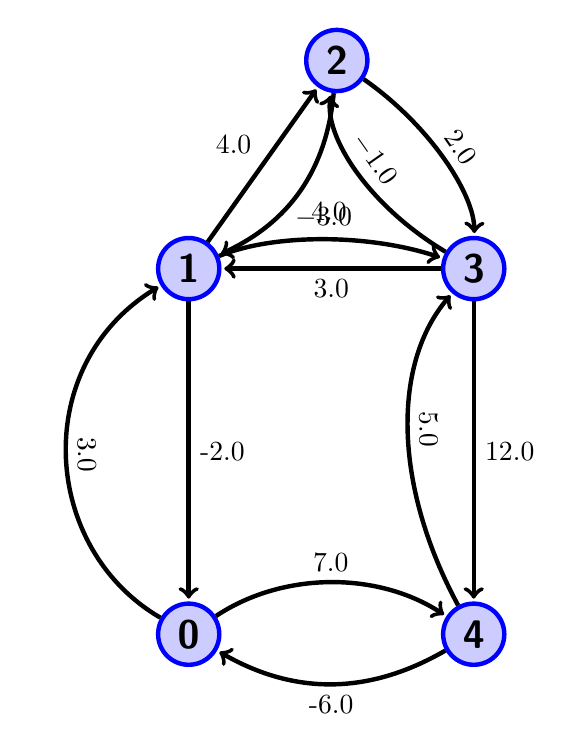
\begin{tikzpicture}[scale=0.90, shorten >=1pt, auto, node distance=3cm, ultra thick,
        node_style/.style={circle,draw=blue,fill=blue!20!,font=\sffamily\Large\bfseries},
        edge_node_style/.style={draw=none,fill=none,midway,sloped},
        selected_node_style/.style={circle,draw=blue,fill=yellow!20!,font=\sffamily\Large\bfseries},
        edge_style/.style={draw=black, ultra thick,->},
        selected_edge_style/.style={draw=yellow, ultra thick,->}]
        \tikzset{quadratic bezier/.style={ to path={(\tikztostart) .. controls($#1!1/3!(\tikztostart)$) and ($#1!1/3!(\tikztotarget)$).. (\tikztotarget)}}}
        
            \node [node_style](n1) at (4.424,-10.602) {0};
            \node [node_style](n2) at (4.424,-5.443) {1};
            \node [node_style](n3) at (6.514,-2.506) {2};
            \node [node_style](n4) at (8.446,-5.443) {3};
            \node [node_style](n5) at (8.446,-10.602) {4};\draw [edge_style] (n1) .. controls (2.331,-9.381) and (2.183,-6.798) .. node [edge_node_style] {$3.0$} (n2);
                    \draw [edge_style] (n2) to[edge label=-2.0] (n1);
            \draw [edge_style] (n3) to[bend left,edge label=4.0] (n2);
            \draw [edge_style] (n2) to[edge label=4.0] (n3);
            \draw [edge_style] (n5) to[bend left,edge label=-6.0] (n1);
            \coordinate (crtl6)  at (6.422,-9.271);
            \draw [edge_style] (n1) .. controls($(crtl6)!1/3!(n1)$) and ($(crtl6)!1/3!(n5)$).. node [edge_node_style] {$7.0$} (n5);
                    \coordinate (crtl7)  at (6.217,-4.7);
            \draw [edge_style] (n2) .. controls($(crtl7)!1/3!(n2)$) and ($(crtl7)!1/3!(n4)$).. node [edge_node_style] {$-3.0$} (n4);
                    \draw [edge_style] (n4) to[edge label=3.0] (n2);
            \coordinate (crtl9)  at (8.47,-3.868);
            \draw [edge_style] (n3) .. controls($(crtl9)!1/3!(n3)$) and ($(crtl9)!1/3!(n4)$).. node [edge_node_style] {$2.0$} (n4);
                    \coordinate (crtl10)  at (6.238,-4.124);
            \draw [edge_style] (n4) .. controls($(crtl10)!1/3!(n4)$) and ($(crtl10)!1/3!(n3)$).. node [edge_node_style] {$-1.0$} (n3);
                    \coordinate (crtl11)  at (6.725,-7.418);
            \draw [edge_style] (n5) .. controls($(crtl11)!1/3!(n5)$) and ($(crtl11)!1/3!(n4)$).. node [edge_node_style] {$5.0$} (n4);
                    \draw [edge_style] (n4) to[edge label=12.0] (n5);
            
        \end{tikzpicture}
    
        \end{center}
        \end{frame}

        
            \begin{frame}
            \frametitle{Floyd-Warshall Algorithm : Iteration 1}
            \begin{center}
            
                \begin{tikzpicture}[xscale=0.60, yscale=0.50]
                    \foreach[count=\n] \x in {3.5, 6.5, 9.5, 12.5, 15.5} \node at (\x, 12) {\n};
                    \foreach[count=\n] \y in {10, 8, 6, 4, 2} \node at ( 1, \y) {\n};
                    \draw[very thick] ( 2.5,0.9)--( 1.9,0.9)--( 1.9,11.1)--( 2.5,11.1);
                    \draw[very thick] (16.5,0.9)--(17.1,0.9)--(17.1,11.1)--(16.5,11.1);
                    
                    \foreach[count=\n] \d in {  0,3,\oo,\oo,7} \dst(1,\n){\d};
                    \foreach[count=\n] \d in {  -2,0,4,-3,5} \dst(2,\n){\d};
                    \foreach[count=\n] \d in {  \oo,4,0,2,\oo} \dst(3,\n){\d};
                    \foreach[count=\n] \d in {  \oo,3,-1,0,12} \dst(4,\n){\d};
                    \foreach[count=\n] \d in {  -6,-3,\oo,5,0} \dst(5,\n){\d};
                    \foreach[count=\n] \d in {  ~,0,~,~,0} \via(1,\n){\d};
                    \foreach[count=\n] \d in {  0,~,0,0,1} \via(2,\n){\d};
                    \foreach[count=\n] \d in {  ~,0,~,0,~} \via(3,\n){\d};
                    \foreach[count=\n] \d in {  ~,0,0,~,0} \via(4,\n){\d};
                    \foreach[count=\n] \d in {  0,1,~,0,~} \via(5,\n){\d};
                \end{tikzpicture}
    
            \end{center}
            \end{frame}
        
            \begin{frame}
            \frametitle{Floyd-Warshall Algorithm : Iteration 2}
            \begin{center}
            
                \begin{tikzpicture}[xscale=0.60, yscale=0.50]
                    \foreach[count=\n] \x in {3.5, 6.5, 9.5, 12.5, 15.5} \node at (\x, 12) {\n};
                    \foreach[count=\n] \y in {10, 8, 6, 4, 2} \node at ( 1, \y) {\n};
                    \draw[very thick] ( 2.5,0.9)--( 1.9,0.9)--( 1.9,11.1)--( 2.5,11.1);
                    \draw[very thick] (16.5,0.9)--(17.1,0.9)--(17.1,11.1)--(16.5,11.1);
                    
                    \foreach[count=\n] \d in {  0,3,7,0,7} \dst(1,\n){\d};
                    \foreach[count=\n] \d in {  -2,0,4,-3,5} \dst(2,\n){\d};
                    \foreach[count=\n] \d in {  2,4,0,1,9} \dst(3,\n){\d};
                    \foreach[count=\n] \d in {  1,3,-1,0,8} \dst(4,\n){\d};
                    \foreach[count=\n] \d in {  -6,-3,1,-6,0} \dst(5,\n){\d};
                    \foreach[count=\n] \d in {  ~,0,2,2,0} \via(1,\n){\d};
                    \foreach[count=\n] \d in {  0,~,0,0,1} \via(2,\n){\d};
                    \foreach[count=\n] \d in {  2,0,~,2,2} \via(3,\n){\d};
                    \foreach[count=\n] \d in {  2,0,0,~,2} \via(4,\n){\d};
                    \foreach[count=\n] \d in {  0,1,2,2,~} \via(5,\n){\d};
                \end{tikzpicture}
    
            \end{center}
            \end{frame}
        
            \begin{frame}
            \frametitle{Floyd-Warshall Algorithm : Iteration 3}
            \begin{center}
            
                \begin{tikzpicture}[xscale=0.60, yscale=0.50]
                    \foreach[count=\n] \x in {3.5, 6.5, 9.5, 12.5, 15.5} \node at (\x, 12) {\n};
                    \foreach[count=\n] \y in {10, 8, 6, 4, 2} \node at ( 1, \y) {\n};
                    \draw[very thick] ( 2.5,0.9)--( 1.9,0.9)--( 1.9,11.1)--( 2.5,11.1);
                    \draw[very thick] (16.5,0.9)--(17.1,0.9)--(17.1,11.1)--(16.5,11.1);
                    
                    \foreach[count=\n] \d in {  0,3,7,0,7} \dst(1,\n){\d};
                    \foreach[count=\n] \d in {  -2,0,4,-3,5} \dst(2,\n){\d};
                    \foreach[count=\n] \d in {  2,4,0,1,9} \dst(3,\n){\d};
                    \foreach[count=\n] \d in {  1,3,-1,0,8} \dst(4,\n){\d};
                    \foreach[count=\n] \d in {  -6,-3,1,-6,0} \dst(5,\n){\d};
                    \foreach[count=\n] \d in {  ~,0,2,2,0} \via(1,\n){\d};
                    \foreach[count=\n] \d in {  0,~,0,0,1} \via(2,\n){\d};
                    \foreach[count=\n] \d in {  2,0,~,2,2} \via(3,\n){\d};
                    \foreach[count=\n] \d in {  2,0,0,~,2} \via(4,\n){\d};
                    \foreach[count=\n] \d in {  0,1,2,2,~} \via(5,\n){\d};
                \end{tikzpicture}
    
            \end{center}
            \end{frame}
        
            \begin{frame}
            \frametitle{Floyd-Warshall Algorithm : Iteration 4}
            \begin{center}
            
                \begin{tikzpicture}[xscale=0.60, yscale=0.50]
                    \foreach[count=\n] \x in {3.5, 6.5, 9.5, 12.5, 15.5} \node at (\x, 12) {\n};
                    \foreach[count=\n] \y in {10, 8, 6, 4, 2} \node at ( 1, \y) {\n};
                    \draw[very thick] ( 2.5,0.9)--( 1.9,0.9)--( 1.9,11.1)--( 2.5,11.1);
                    \draw[very thick] (16.5,0.9)--(17.1,0.9)--(17.1,11.1)--(16.5,11.1);
                    
                    \foreach[count=\n] \d in {  0,3,-1,0,7} \dst(1,\n){\d};
                    \foreach[count=\n] \d in {  -2,0,-4,-3,5} \dst(2,\n){\d};
                    \foreach[count=\n] \d in {  2,4,0,1,9} \dst(3,\n){\d};
                    \foreach[count=\n] \d in {  1,3,-1,0,8} \dst(4,\n){\d};
                    \foreach[count=\n] \d in {  -6,-3,-7,-6,0} \dst(5,\n){\d};
                    \foreach[count=\n] \d in {  ~,0,4,2,0} \via(1,\n){\d};
                    \foreach[count=\n] \d in {  0,~,4,0,1} \via(2,\n){\d};
                    \foreach[count=\n] \d in {  2,0,~,2,2} \via(3,\n){\d};
                    \foreach[count=\n] \d in {  2,0,0,~,2} \via(4,\n){\d};
                    \foreach[count=\n] \d in {  0,1,4,2,~} \via(5,\n){\d};
                \end{tikzpicture}
    
            \end{center}
            \end{frame}
        
            \begin{frame}
            \frametitle{Floyd-Warshall Algorithm : Iteration 5}
            \begin{center}
            
                \begin{tikzpicture}[xscale=0.60, yscale=0.50]
                    \foreach[count=\n] \x in {3.5, 6.5, 9.5, 12.5, 15.5} \node at (\x, 12) {\n};
                    \foreach[count=\n] \y in {10, 8, 6, 4, 2} \node at ( 1, \y) {\n};
                    \draw[very thick] ( 2.5,0.9)--( 1.9,0.9)--( 1.9,11.1)--( 2.5,11.1);
                    \draw[very thick] (16.5,0.9)--(17.1,0.9)--(17.1,11.1)--(16.5,11.1);
                    
                    \foreach[count=\n] \d in {  0,3,-1,0,7} \dst(1,\n){\d};
                    \foreach[count=\n] \d in {  -2,0,-4,-3,5} \dst(2,\n){\d};
                    \foreach[count=\n] \d in {  2,4,0,1,9} \dst(3,\n){\d};
                    \foreach[count=\n] \d in {  1,3,-1,0,8} \dst(4,\n){\d};
                    \foreach[count=\n] \d in {  -6,-3,-7,-6,0} \dst(5,\n){\d};
                    \foreach[count=\n] \d in {  ~,0,4,2,0} \via(1,\n){\d};
                    \foreach[count=\n] \d in {  0,~,4,0,1} \via(2,\n){\d};
                    \foreach[count=\n] \d in {  2,0,~,2,2} \via(3,\n){\d};
                    \foreach[count=\n] \d in {  2,0,0,~,2} \via(4,\n){\d};
                    \foreach[count=\n] \d in {  0,1,4,2,~} \via(5,\n){\d};
                \end{tikzpicture}
    
            \end{center}
            \end{frame}
        
    \end{document}
    
